%%%% Better Poster latex template example v1.0 (2019/04/04)
%%%% GNU General Public License v3.0
%%%% Rafael Bailo
%%%% https://github.com/rafaelbailo/betterposter-latex-template
%%%%
%%%% Original design from Mike Morrison
%%%% https://twitter.com/mikemorrison
\documentclass[poster,fleqn]{betterposter}
\usepackage[T1]{fontenc}
\usepackage[colorlinks=true, urlcolor=white]{hyperref}
\usepackage{tikz}
\usepackage{enumerate}
\usepackage{setspace}
\usepackage{pgf}
\usepackage{lmodern}
\usepackage{import}
\usepackage{xfakebold}
%\usepackage{inconsolata}

%%%% Uncomment the following commands to customise the format

%% Setting the width of columns
% Left column
\setlength{\leftbarwidth}{0.25\paperwidth}
% Right column
\setlength{\rightbarwidth}{0.25\paperwidth}

%% Setting the column margins
% Horizontal margin
\setlength{\columnmarginvertical}{0.04\paperheight}
% Vertical margin
\setlength{\columnmarginhorizontal}{0.02\paperheight}
% Horizontal margin for the main column
\setlength{\maincolumnmarginvertical}{0.05\paperheight}
% Vertical margin for the main column
\setlength{\maincolumnmarginhorizontal}{0.05\paperheight}

%% Changing font sizes
% Text font
%\renewcommand{\fontsizestandard}{\fontsize{28}{35} \selectfont}
% Main column font
%\renewcommand{\fontsizemain}{\fontsize{28}{35} \selectfont}
% Title font
%\renewcommand{\fontsizetitle}{\fontsize{28}{35} \selectfont}
% Author font
%\renewcommand{\fontsizeauthor}{\fontsize{28}{35} \selectfont}
% Section font
%\renewcommand{\fontsizesection}{\fontsize{28}{35} \selectfont}

%% Changing font sizes for a specific text segment
% Place the text inside brackets:
% {\fontsize{28}{35} \selectfont Your text goes here}

%% Changing colours
% Background of side columns
%\renewcommand{\columnbackgroundcolor}{black}
% Font of side columns
%\renewcommand{\columnfontcolor}{gray}
% Background of main column
%\renewcommand{\maincolumnbackgroundcolor}{empirical}
%\renewcommand{\maincolumnbackgroundcolor}{theory}
%\renewcommand{\maincolumnbackgroundcolor}{methods}
%\renewcommand{\maincolumnbackgroundcolor}{intervention}
\renewcommand{\maincolumnbackgroundcolor}{uiucindustrial}
\newcommand{\romani}[1]{\textcolor{altgeldorange}{\textbf{(#1)}}}
\newcommand{\capt}[1]{\setstretch{1.0}\textcolor{gray}{\fontsizestandard #1}}
% Font of main column
%\renewcommand{\maincolumnfontcolor}{gray}


\tikzstyle{blurb} = [rectangle, rounded corners, text centered, draw=black, text width = .99\textwidth, anchor = west, fill = white]

\tikzstyle{main} = [rectangle, rounded corners, text centered, 
draw = white, text width = .315\textwidth, anchor = west, fill = white]

\tikzstyle{logo} = [rectangle, text centered, text width = .3\linewidth]

\begin{document}
\betterposter{
%%%%%%%% MAIN COLUMN

\maincolumn{
\vspace{-2.5cm}
\begin{center}
ARFC: \textbf{Advanced Reactors} and \textbf{Fuel Cycles}\\
\fontsizetitle
PI: {\textbf{Prof. Katy Huff}}, \href{mailto:kdhuff@illinois.edu}{\underline{kdhuff}@\underline{illinois.edu}}\\
\vspace{-2cm}\rule{\textwidth}{5pt}\vspace{2cm}
\end{center}

\fontsizesection
\begin{tikzpicture}
\iftrue
\node (multiphysics) [main, xshift=-3cm] {
\textcolor{black}{
\\{\fontsizetitle Coupled Multiphysics of Advanced Reactors}\\
\vspace{-25pt}\rule{\textwidth}{5pt}\\
\fontsizesection
\vspace{.5cm}
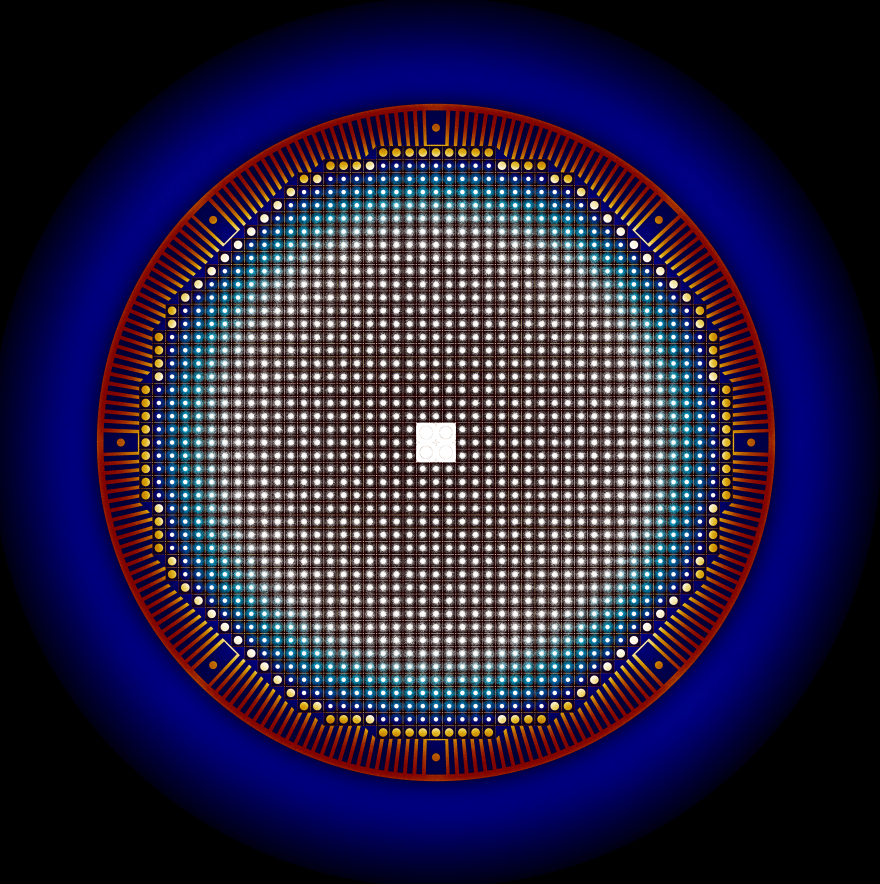
\includegraphics[width = \textwidth]{img/multiphysics.png}\\
}
};
\node (fuelcycle) [main, right of = multiphysics, xshift = 17.65cm] {
\textcolor{black}{
\\{\fontsizetitle Nuclear Fuel Cycle Analysis}\\
\vspace{-20pt}\rule{\textwidth}{5pt}\\
\fontsizesection
\vspace{1.5cm}
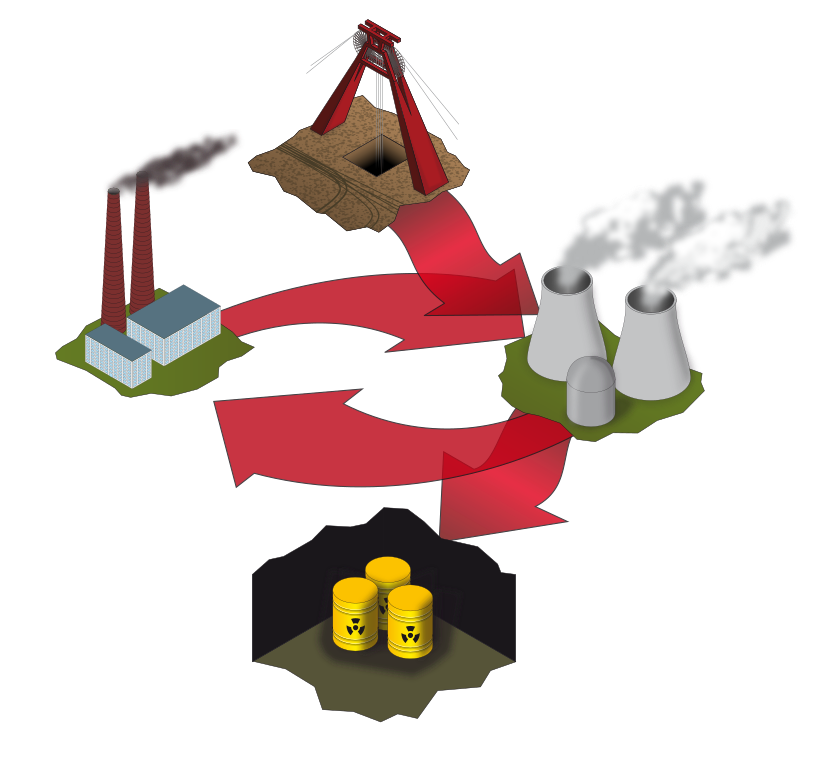
\includegraphics[width=\textwidth]{img/nfc.png}\\
\vspace{7pt}
}
};
\node (compute) [main, right of = fuelcycle, xshift = 17.65cm] {
\textcolor{black}{
\\{\fontsizetitle Advanced Computation}\\
\vspace{-25pt}\rule{\textwidth}{5pt}\\
\fontsizesection
\vspace{17pt}
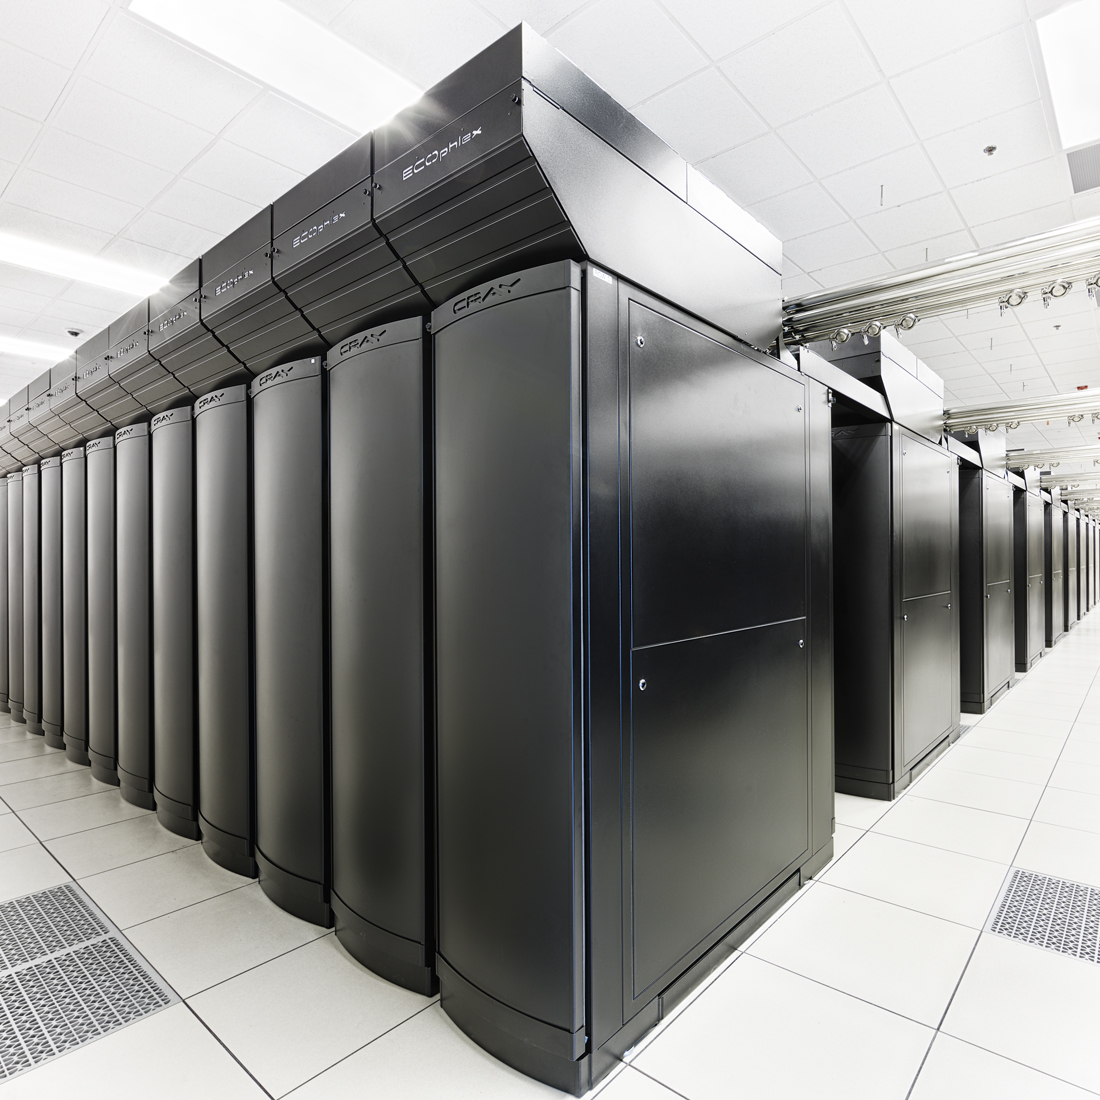
\includegraphics[width=\textwidth]{img/bw_cropped.jpg}\\
\vspace{5pt}
}
};
\fi
\iffalse
\node (diagram) [blurb, xshift = -3cm] {
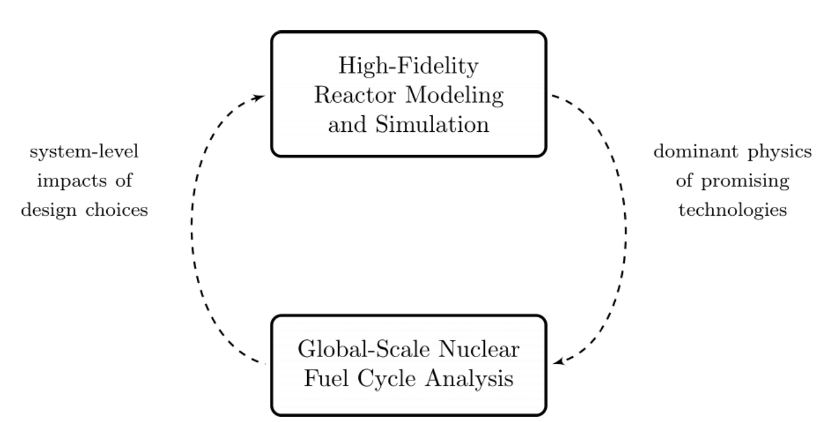
\includegraphics[width = \linewidth]{img/diagram.png}
};
%yshift is 21 for including this
\fi
\node (logos) [blurb, yshift = -19cm, xshift = -3cm] {\vspace{5pt}
\textcolor{black}{
\\{\fontsizetitle Open-Source Nuclear Research Codes}\\
\vspace{-20pt}\rule{\textwidth}{5pt}\\
\vspace{25pt}
\begin{minipage}{.2\linewidth}
    
\includegraphics[width = \linewidth]{img/openmc_logo.png}\\
    \vspace{5pt}
    
\includegraphics[width = \linewidth]{img/rollo-logo.png}
\end{minipage} 
\begin{minipage}{.2\linewidth}
    
\includegraphics[width =.8\linewidth]{img/pyne.png}
    \vspace{10pt}
\end{minipage}
\begin{minipage}{.2\linewidth}
    
\includegraphics[width=.8\linewidth]{img/ghastly.png}
\end{minipage}
\begin{minipage}{.2\linewidth}
    
\includegraphics[width=\linewidth]{img/cyclus.png}\\
    \vspace{20pt}
    \textcolor{altgeldorange!100}{\textbf{\fontsizemoltres{\texttt{Moltres}}}}\\\vspace{-15pt}
\end{minipage}
}
};
\end{tikzpicture}

\vspace{1.5cm}
\begin{minipage}{.235\linewidth}
    \centering
    
\includegraphics[width=.8\linewidth]{img/qrcode.eps}
    \href{https://arfc.github.io/}{\fontsizesection\underline{https://arfc.github.io/}}
\end{minipage}
\vspace{-1cm}
\begin{minipage}{0.72\linewidth}
    \hspace{.5cm}
    \begin{tikzpicture}
    \vspace{-1cm}
        \node (logos) [blurb] {
        \begin{minipage}{.3\linewidth}
        `   %https://www.energy.gov/department-energy-logo-and-branding-guidelines
            
\includegraphics[width = \linewidth]{img/doe.png}
        \end{minipage}
        \begin{minipage}{.3\linewidth}
            %https://commons.wikimedia.org/wiki/File:NNSA_Logo.png
            
\includegraphics[width = \linewidth]{img/nnsa.png}
        \end{minipage}
        \begin{minipage}{.3\linewidth}
            % top left https://en.m.wikipedia.org/wiki/File:US-NuclearRegulatoryCommission-Logo.svg
            
\includegraphics[width = \linewidth]{img/nrc.png}
        \end{minipage}\\
        \vspace{1cm}
        \begin{minipage}{.3\linewidth}
        `   %https://www.moltexenergy.com/partners/ornl-logo/
            
\includegraphics[width = \linewidth]{img/ornl.png}
        \end{minipage}
        \begin{minipage}{.3\linewidth}
            %https://commons.wikimedia.org/wiki/File:Argonnelablogo.PNG
            
\includegraphics[width = \linewidth]{img/anl.png}
        \end{minipage}
        \begin{minipage}{.3\linewidth}
        \hspace{3.25cm}
            % https://inl.gov/logos-videos-images/
            
\includegraphics[height = .5\linewidth]{img/inl.png}
        \end{minipage}
        };
    \end{tikzpicture}
\end{minipage}

\vspace{2cm}
\begin{minipage}{\textwidth}
    
    \begin{tikzpicture}
    \node (refs) [blurb] {\textcolor{black}{\fontsizetitle
    \vspace{-50pt}\\{References}\\\vspace{-75pt}\\
    \rule{\textwidth}{5pt}\\
    \fontsizerefs
    \begin{itemize}[leftmargin = 4cm, rightmargin = 5cm]
        \item[[1\hspace{-4pt}]]\quad S. M. Park, “Advancements in Moltres for Time-Dependent Multiphysics Molten Salt Reactor Modeling,” Doctoral Dissertation, University of Illinois Urbana-Champaign, Urbana, 2025.\\
        \item[[2\hspace{-4pt}]] \quad A. M. Bachmann, “Investigation of the impacts of deploying reactors fueled by high-assay low enriched uranium,” Doctoral Dissertation, University of Illinois at Urbana-Champaign, 2023.\\
        \item[[3\hspace{-4pt}]] \quad G. J. Y. Chee, “Fluoride-Salt-Cooled High Temperature Reactor Design Optimization with Evolutionary Algorithms,” Doctoral Dissertation, University of Illinois at Urbana-Champaign, Urbana, 2022.\\
        \item[[4\hspace{-4pt}]]\quad Z. Richter, E. Davidson, S. Skutnik, and M. Munk, “MODELING AND SIMULATION OF AN XE-100 TYPE PEBBLE BED GAS-COOLED REACTOR WITH SCALE,” Technical Report ORNL/TM-2023/2959, 2023.\\
    \end{itemize}
    }
    };
\end{tikzpicture}
\end{minipage}

}{
}

}{
%%%%%%%% LEFT COLUMN
\vspace{-2.5cm}
\begin{tikzpicture}
    \node (park) [blurb] {
    \\{\fontsizetitle Moltres}\\
    \vspace{-20pt}\rule{\textwidth}{5pt}\\
    \fontsizesection
    S$_N$-D method for accurate time-dependent control rod modeling in Moltres, an open-source MOOSE application for the simulation of molten salt reactors [1]\iffalse\cite{park}\fi.\\
    \begin{center}
        \includegraphics[width = .4\textwidth]{img/msre-full-0-power.png}
        \hspace{2cm}
        \includegraphics[width = .4\textwidth]{img/msre-full-123-power.png}
        \\
        \capt{MSRE full core scalar flux error as calculated with pure diffusion, $S_N-D$, and OpenMC for all control rods removed (left) and all control rods inserted (right)}
    \end{center}

    };
    \node (bachmann) [blurb, below of = park, yshift=-19.25cm] {
    \\{\fontsizetitle OpenMCyclus}\\
    \vspace{-20pt}\rule{\textwidth}{5pt}\\
    \fontsizesection
    Reactor-physics informed fuel cycle analysis on the impacts of deploying HALEU-fueled reactors using OpenMCyclus, a coupling of OpenMC with Cyclus [2]\iffalse\cite{bachmann}\fi.\\
    \begin{center}
    \begin{minipage}{.45\textwidth}
    \vspace{1cm}
        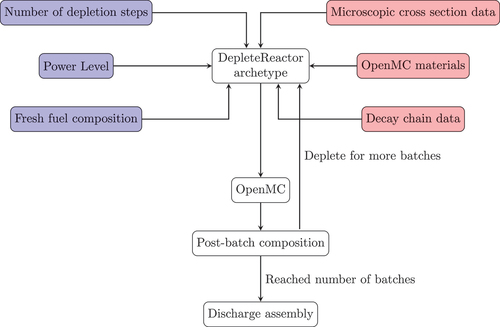
\includegraphics[width = \textwidth]{img/bachmann.jpg}\\
    
        \capt{Depletion methodology in OpenMCyclus. Blue comes from Cyclus and Red is provided through user-inputs.}
    \end{minipage}
    \hspace{1cm}
    \begin{minipage}{.45\textwidth}
    \vspace{0cm}
        \vspace{.5cm}
        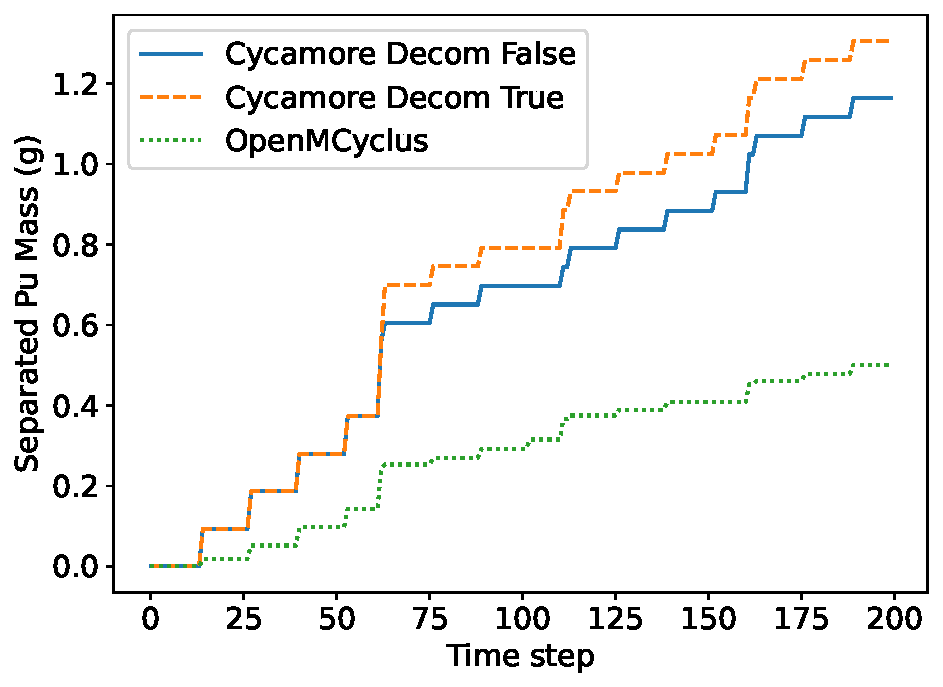
\includegraphics[width = \textwidth]{img/comparison_pu_cumulative.pdf}\\
        \vspace{-1cm}
        
        \capt{Comparison of the cumulative mass of separated plutonium traded after using the OpenMCyclus and Cycamore reactor.}
    \end{minipage}
    \end{center}
    };
    \node (chee) [blurb, below of = bachmann, yshift = -20.75cm] {
    \\{\fontsizetitle ROLLO}\\
    \vspace{-20pt}\rule{\textwidth}{5pt}\\
    \fontsizesection
    Evolutionary algorithm techniques applied to optimize nuclear reactor design by coupling nuclear software to the DEAP evolutionary algorithm driver [3] \iffalse\cite{chee}\fi.
    \begin{center}
    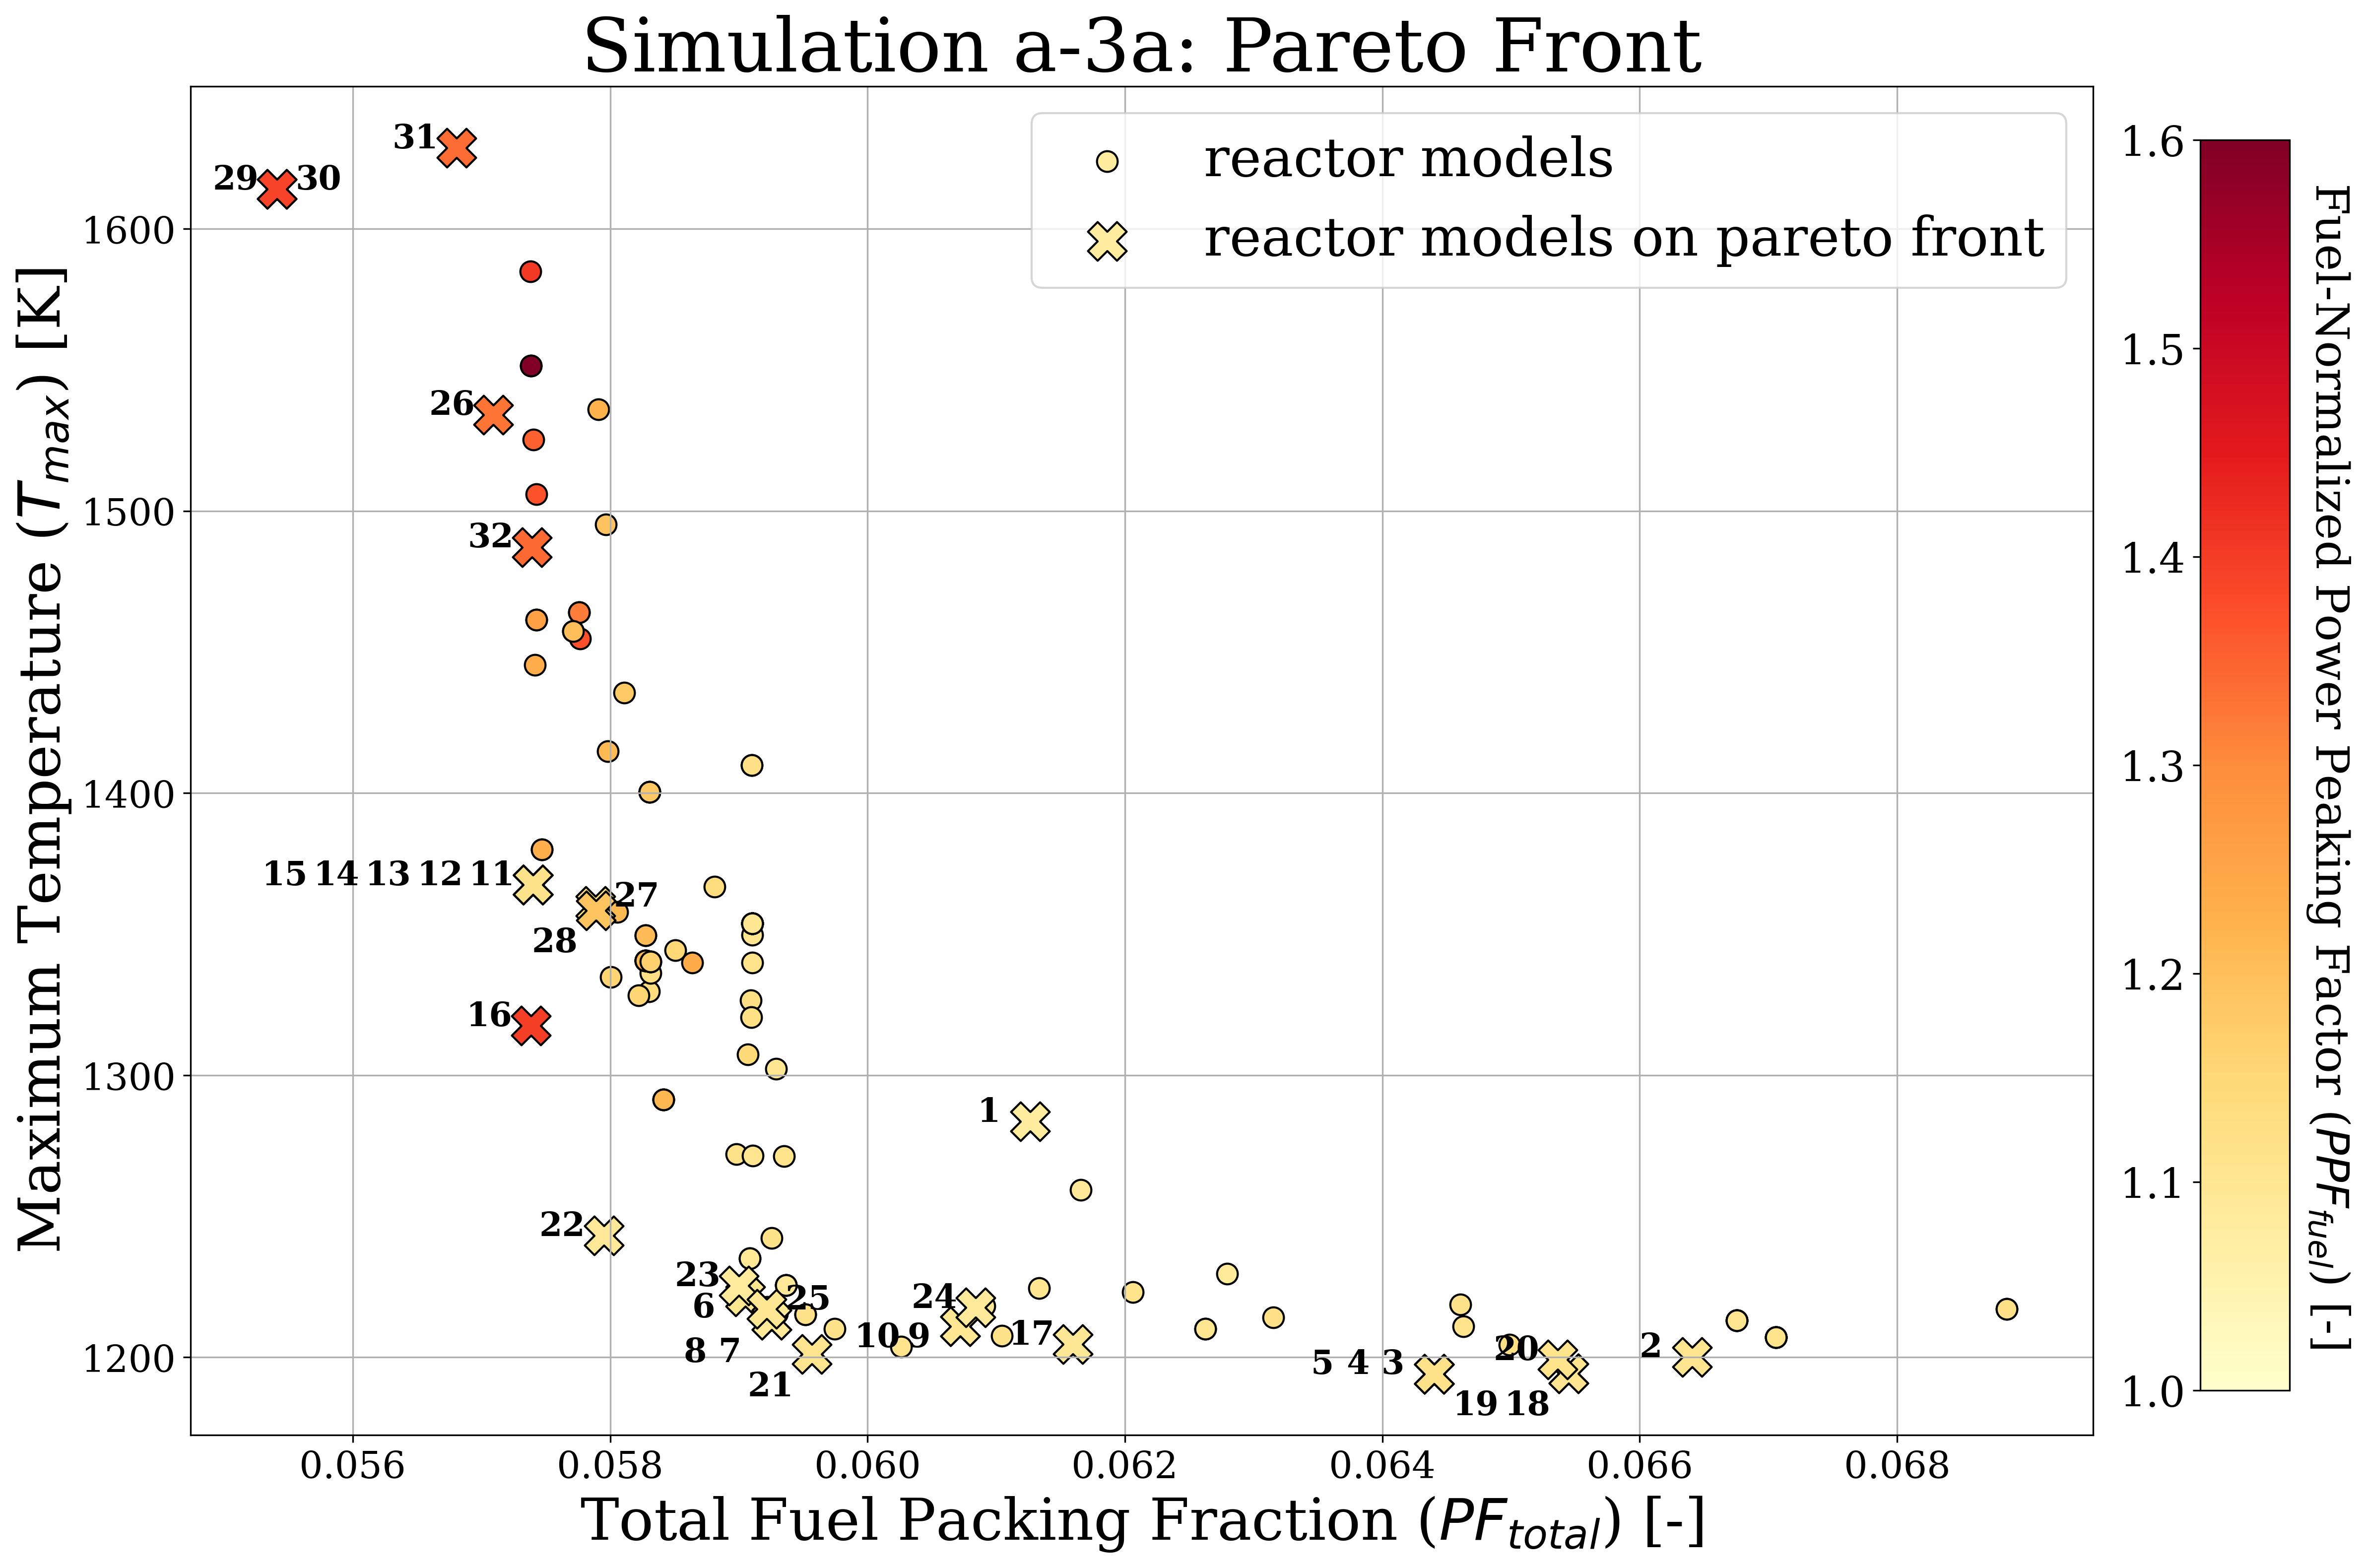
\includegraphics[width = .7\textwidth]{img/assem-obj-3-2d.png}
    \\
    \capt{Triple-objective optimization to minimize total fuel packing fraction, max temp, and fuel-normalized power peaking factor in the one-third assembly}
    \end{center}
    };
\end{tikzpicture}
%% This fills the space between the content and the logo
\vfill

%% Institution logo
\begin{center}


\includegraphics[height=0.28\textwidth]{img/UIUC_Logo.png}\hspace{5cm}

\includegraphics[height=0.28\textwidth, trim={0 .5cm 0 .5cm}]{img/arfc_atom.png}

\end{center}

}{
\vspace{-2.5cm}
\begin{tikzpicture}
    \node (physics) [blurb] {
    \vspace{5pt}
    \textcolor{black}{
    \\{\fontsizetitle Physics of Advanced Reactors}\\
    \vspace{-20pt}\rule{\textwidth}{5pt}\\
    \fontsizesection
    Variance reduction methods for time-dependent Monte Carlo neutron transport. \\
        \vspace{20pt}
    Updated models of DNP group parameters for Molten Salt Reactors. \\
        \vspace{20pt}
    Computational modeling of flowing pebble-bed reactor systems.
        \begin{center}
        \begin{minipage}{.2\linewidth}
            
\includegraphics[height = 3\textwidth]{img/ghastly1.png}
        \end{minipage}
        \hspace{.5cm}
        \begin{minipage}{.2\linewidth}
            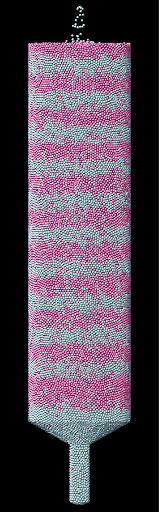
\includegraphics[height = 3\textwidth]{img/ghastly2.png}
        \end{minipage}
        \hspace{.5cm}
        \begin{minipage}{.2\linewidth}
            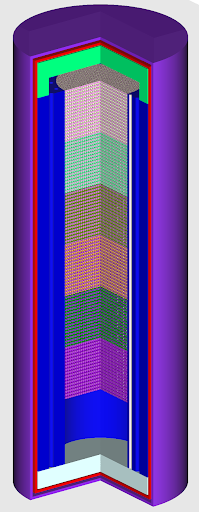
\includegraphics[height = 3\textwidth]{img/ghastly3.png}
        \end{minipage}\\\vspace{10pt}
        \capt{Simulation of a generic pebble bed HTGR core being filled (left) and online pebble recirculation (middle) using LAMMPS, 
        and a Xe-100-like full-core pebble bed HTGR (right) using SCALE [4].}\iffalse{\fontsizestandard\cite{richter}.}\fi
        \end{center}
    }
    };
    %\node (cycles) [blurb, below of = physics, yshift = -35.25cm] {
    \node (cycles) [blurb, below of = physics, yshift = -35.70cm] {
    \vspace{5pt}
    \textcolor{black}{
    \\{\fontsizetitle Fuel Cycle and Energy System Optimization}\\
    \vspace{-20pt}\rule{\textwidth}{5pt}\\
    \fontsizesection
    Modeling and simulating scaled isotopic consequences of deploying Accelerators Driven Systems.\\
        \vspace{20pt}
    Techno-economic analysis of hybrid nuclear renewable energy systems (e.g. hydrogen microgrids).
        \begin{center}
        \begin{minipage}{.7\textwidth}
            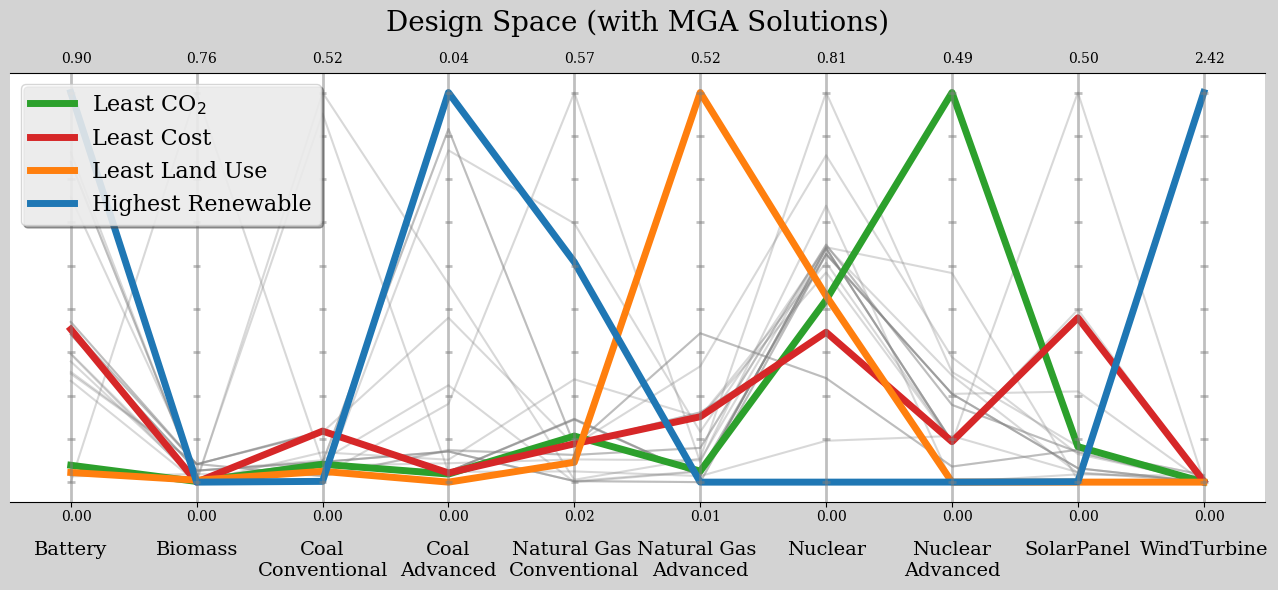
\includegraphics[width = \textwidth]{img/osier.png}
        \end{minipage}\\
        \vspace{10pt}\\
        \capt{The design space for a four objective problem including alternative solutions suggested by MGA.}
        \end{center}\\
        \vspace{20pt}
    Fuel cycle transition scenarios for advanced reactors.
        \begin{center}
        \begin{minipage}{.6\textwidth}
            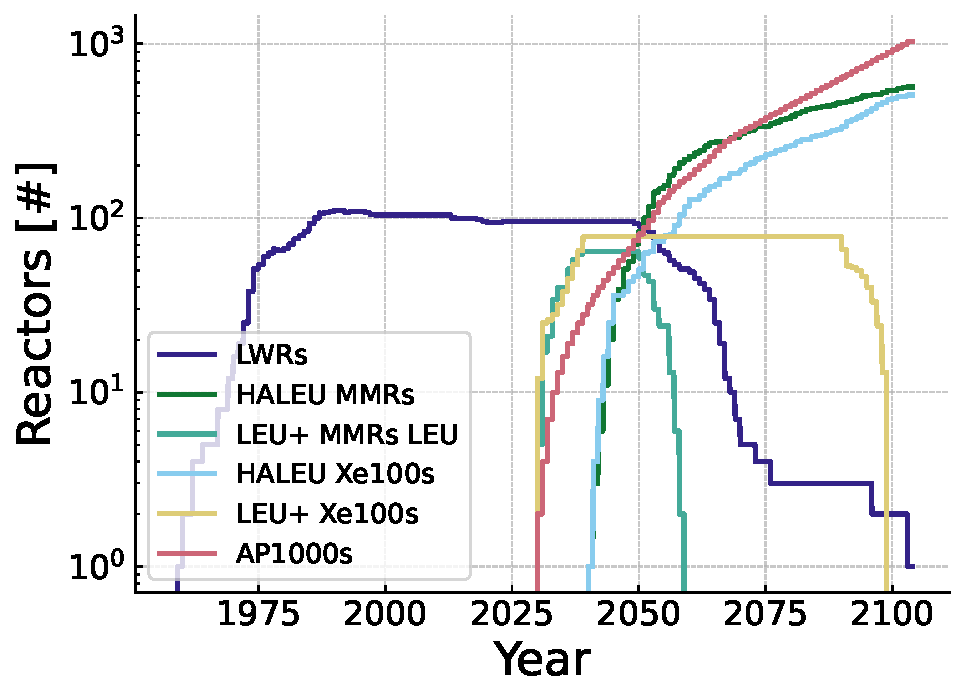
\includegraphics[width = \textwidth]{img/multi_dg2_reactors.pdf}
        \end{minipage}\\
        \vspace{10pt}\\
        \capt{Greedy AP1000 deployment along with Xe-100s and MMRs fueled by LEU+ and HALEU fuel.}
        \end{center}
    }
    };
\end{tikzpicture}
}
\end{document}
